\documentclass[12pt, a4paper, titlepage]{article}
\usepackage[spanish]{babel}
\usepackage[utf8]{inputenc}
%%Imágenes
\usepackage{graphicx}
%%Colores de texto
\usepackage{xcolor}
%%Links
\usepackage[hidelinks]{hyperref}

\definecolor{guindapoli}{RGB}{102, 0, 51}
\definecolor{azulescom}{RGB}{0, 0, 102}

\begin{document}
	
	%PORTADA
	\begin{titlepage}	
		
		\vspace*{-1.5in}
		
		\begin{figure}[htb]
			\begin{center}
				
\includegraphics[width=4cm]{./imagenes/logoipn.png}
			\end{center}
		\end{figure}
		
		\begin{center}
			
			\begin{LARGE}
				\textcolor{guindapoli}{INSTITUTO POLITÉCNICO NACIONAL}\\
			\end{LARGE}	
			
			\vspace*{0.2in}
			
			\begin{Large}
				\textcolor{azulescom}{ESCUELA SUPERIOR DE CÓMPUTO}\\
			\end{Large}		
			
			\vspace*{0.4in}
			
			\begin{large}
				Trabajo Terminal I.\\
			\end{large}
			
			\vspace*{0.2in}
			
			\begin{Large}
				\textbf{Autentificación Mediante Chaffing And Winnowing En El Protocolo HTTP}\\
			\end{Large}
			
			\vspace*{0.2in}
			
			\begin{large}
				2018-B003.\\
			\end{large}
			
			\vspace*{0.2in}
			
			\rule{80mm}{.1mm}\\
			\vspace*{0.1in}
			
			\begin{large}
				\begin{center}
					Integrantes:\\
					Carrillo Fernández Jerry\\
					Blancas Pérez Bryan Israel\\
					Morales González Diego Arturo\\
					Paredes Hernández Pedro Antonio\\
				\end{center}
			\end{large}
			
			\begin{large}
				Directores:\\
				Moreno Cervantes Axel Ernesto\\
				Díaz Santiago Sandra\\
			\end{large}
			
		\end{center}
	
	\end{titlepage}

	\begin{appendix}
		%%Índice
		\href{}{\renewcommand*\contentsname{{\textcolor{azulescom}{Índice.}}}}
		\tableofcontents
		\newpage
		%%índice de figuras
		\renewcommand*\listfigurename{{\textcolor{azulescom}{Índice de figuras.}}}
		\listoffigures
		\newpage
		%%Índice de tablas
		\newpage
		\renewcommand*\listtablename{{\textcolor{azulescom}{Índice de cuadros.}}}
		\listoftables
	\end{appendix}
	\newpage
	

	\section{\textcolor{azulescom}{Introducción.}}
		\subsection{Planteamiento del problema.}
		\subsection{Justificación.}
		\subsection{Objetivos.}
		\subsection{Metodología.}
		\subsection{Estado del Arte.}
	\newpage
	\section{\textcolor{azulescom}{Marco Teórico.}}
		\subsection{Formato a decidir.}
	\newpage
	\section{\textcolor{azulescom}{Análisis.}}
		\subsection{Prototipo I.}
			\subsubsection{Descripción.}
				En este prototipo se busca la creación de una extensión de Google Chrome, que sea capaz de interceptar una petición HTTP hecha por el navegador.
			\subsubsection{Herramientas a usar.}
			
\subsubsection{Estudio de requerimientos.}
				
				\paragraph{Requerimientos Funcionales.\\ \\}
				
				{\setlength{\parindent}{12pt}
				\textbf{PI\_RF1. Interceptar petición HTTP.} La extensión deberá interceptar la petición HTTP del navegador, en cuanto el usuario realice alguna a través del navegador.\\

				\textbf{PI\_RF2. Deshabilitar extensión.} El usuario podrá deshabilitar la extensión, para que ésta no vigile su actividad en el navegador.\\
				
				\textbf{PI\_RF3. Habilitar extensión.} El usuario podrá habilitar la extensión, para que ésta vigile constantemente cuando éste realice una petición HTTP.
				}
				
				\paragraph{Requerimientos no Funcionales.\\ \\}
				{\setlength{\parindent}{12pt}
				
				\textbf{PI\_RNF1. Plataforma de implementación.} La extensión será implementada en el navegador Google Chrome.\\
				
				\textbf{PI\_RNF2. Versión del navegador} La extensión funcionará a partir de la versión 65.0.3325.181.\\
				
				\textbf{PI\_RNF3. Tecnologías para la interfaz de usuario} Para el sistema se hará uso de HTML, JavaScript, CSS, JSON.\\
				\footnote{Checar si es necesario especificar que debe estar habilitado JavaScript y si sería Funcional o No funcional}
				
				}\newpage
			
			\subsubsection{Reglas del negocio.\\}
				{\setlength{\parindent}{12pt}
					
					\textbf{PI\_RN1. Confidencialidad de la actividad web.} En cuando el cliente lo indique por medio de la IU, la extensión deberá dejar de vigilar la actividad que el usuario realice en el navegador.\\
					
				}\newpage
	\newpage
	\section{\textcolor{azulescom}{Desarrollo.}}
		\subsection{Prototipo I.}
			\subsubsection{Diagrama de casos de uso.}
			Diagrama de casos de uso general para el prototipo I.
			\begin{figure}[htb]
				\begin{center}
					\label{fig1} 
					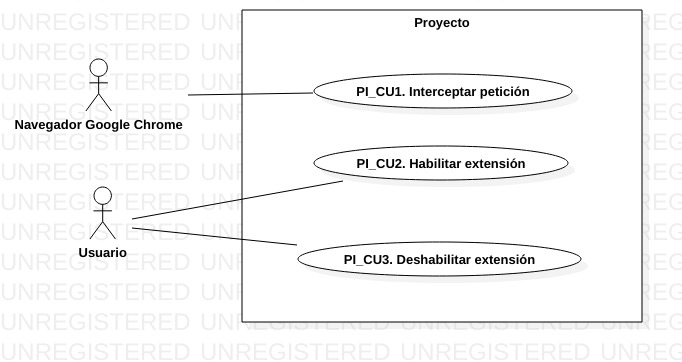
\includegraphics[width=17cm]{./imagenes/UCD_1.jpg}
					\caption{Diagrama de casos de uso.}
				\end{center}
			\end{figure}
			\subsubsection{Descripción de casos de uso.}
			\subsubsection{Diagrama de flujo.}
			\subsubsection{Flujo de datos.}
			\subsubsection{Diagrama de clases.}
			\subsubsection{Diagrama de secuencia.}
			\subsubsection{Interfaz de usuario.}
			\subsubsection{Requisitos de diseño.}
			
\end{document}
